\documentclass[a4paper,12pt,titlepage]{article}
\usepackage{graphicx}
\usepackage[hidelinks]{hyperref}
\usepackage{listings}
%\setcounter{tocdepth}{1}
\usepackage{float}
\usepackage[T1]{fontenc}




\DeclareGraphicsExtensions{.png}
%\graphicspath{ {./images/} }

\begin{document}
\begin{titlepage}
	\begin{center}
		
		\begin{figure}[t]
			\centering
			
\includegraphics[width=350px]{UP_Logo.png}
		\end{figure}		
		
		\textbf{\LARGE COS301 Mini Project Functional \\Architecture Requirements\\}
		
		\vspace{1 cm}
		
		\LARGE{\textbf{Group Name: }Group 7\_a}
		
		%\begin{minipage}{0.4\textwidth}

		\begin{flushright} \large
			Roger Tavares \emph10167324\newline
			Thinus Naude \emph13019602 \newline
			Kabelo Kgwete \emph11247143\newline
			Sylvester Mpanganer \emph11241617\newline
			Maphuti Setati \emph12310043\newline
			Ruth Ojo \emph12042804\newline
			Axel Ind \emph12063178\newline
			Lindelo Mapumulo \emph12002862\newline
			Maria Qumalo \emph29461775\newline
		\end{flushright}
		%\end{minipage}
		
		\vfill
		
		\textbf{Git repository link:\\}
		\url{https://github.com/thinusn/COS301MiniProjectArchitectureRequirements}
		
		\vfill
		
		{\LARGE Final Version}
		\\
		{\large \today}		
		
		
	\end{center}
\end{titlepage}



%-----------------TABLE OF CONTENT-----------------
\newpage
\tableofcontents


%-----------------BASIC INTRODUCTION-----------------
\newpage
\section{Introduction}

This document was compiled by our group during our meetings and was produced as a whole by the team. \bigskip

This document contains specifications of the software architecture requirements. This is the infrastructure upon which the application functionality will be developed. \bigskip

The following non-functional requirements are addressed in depth with supporting diagrams(when necessary):

\begin{itemize}
	\item Quality requirements.
	\item Integration and access channel requirements.
	\item Architectural constraints
	\item Architectural patterns or styles
	\item Architectural tactics or strategies
	\item Use of reference architectures and frameworks
	\item Access and integration channels
	\item Technologies
\end{itemize}

%-----------------PARTS TO EDIT-----------------
\newpage

\section{Architecture Requirements}
\subsection{Architectural Scope} %Maria
This section discusses the boundaries and extent or range of view, outlook, applications, operations or effectiveness the system software architectur needs to address. 
More spesificaly we will be looking at the following three topics in depth. Persistence, Reporting and Process execution.

%Persistence
\subsubsection{Persistence}
	Buzz Space needs to be percistant in order for states to be stored and outlive the many
	processes done. It will do so by making use of the following:

		\begin{itemize}
			\item Databases, to store and retrieve user accounts data and information.
			\item Java Data Objects (JDO), a specification of Java object persistence. With it's great
			 transparency feature of the persistence services to the domain model.
			\item System prevalence, a technique that joins system images and transaction journals to achieve percistancey.
		\end{itemize}
	
		%Process execution
	\subsubsection{Reporting}
	It is crucial that the Buzz Space gives the user some sort of reporting and feed back after activities such as successful posts, voting(either up or down), deleted or hidden posts, read and unread posts or any other change of state. This will be achieved by sending the user an email to notify him of any changes. 
	
			 
	%Process execution
	\subsubsection{Process execution}
	Process infrastructure and execution deals with the essential operation components, such as policies, processes, equipment, data and internal operations, for overall effectiveness. In providing a good Process infrastructure for the Buzz Space system, we aim to:
	\begin{itemize}
  \item	Reduce duplication of effort
  \item	Ensure adherence to standards (both coding and design)
  \item	Enhance the flow of information throughout an the system
  \item	Promote adaptability necessary for a changeable environment (Including the different human access channels.)
  \item	Ensure interoperability among organizational and external entities
  \item	Maintain effectiveness
	\end{itemize}

						

\newpage
\subsection{Critical Quality Requirements}
\subsubsection{Scalability}%Ruth
	\subsubsection*{Description}
	Scalability is an essential aspect of a system and is the ability of a system to be easily enlarged in order to accommodate a growing amount of work.
	\subsubsection*{Justification}
	 As the Buzz System should allow for more than a million concurrent users, the system must be able to handle that.
	\subsubsection*{Mechanism}
		\begin{enumerate}
			\item Strategy:\\\\
			Scalability can be achieved by:
			\begin{itemize}
			\item Clustering: using more resources by running many instances of the application over a cluster of servers or instances.
			\item Load Balancing: Spread the systems load across time or across resources through scheduling or queueing. In the case that the limit for a server has been reached, a new instance will have to be created in order to handle the number of increasing requests. On the other hand, if the usage of a server is way below the capacity, the number of instances will have to be reduced.\\\\
			In terms of databases:
			\item Caching: to ensure no duplication or repeated retrieval of frequent objects or queries; a separate module can facilitate caching; thus system resources will not be used up unnecessarily.
			 \end{itemize}
			\item Architectural Pattern(s):
			\begin{itemize}
			\item Blackboard Architectural Pattern
				\begin{itemize}
					\item Makes used of a spaced-based architecture, making it easy to add a new knowledge source or update an existing knowledge source.
				 \end{itemize}
			 \end{itemize}
		\end{enumerate}

\subsubsection{Security}%Kabelo
	\subsubsection*{Description}
	Security includes the securing of confidential data stored from unauthorized access and modification. For BuzzSpace, this means:
	\begin{itemize}
		\item Ensuring only genuine users may have access to the system’s data. 
		\item Different levels of access should be provided to users.
		\item Securing vulnerabilities that may exist in the application.
	\end{itemize}	
	\subsubsection*{Justification}
	 Security is a crucial aspect of the system. Poor security design and implementation can compromise the data stored by the system and hackers with malicious intentions can succeed to gain access to sensitive information. Using a combination of security strategies and patterns, we can prevent unauthorized users from accessing sensitive information or cause damage to the system.
	\subsubsection*{Mechanism}
		\begin{enumerate}
			\item Strategy:\\\\
			Security can be achieved by using:
			\begin{itemize}
			\item Authentication: This is the process that ensures and confirms a user’s identity.
			\item Encryption: This process converts sensitive data into another form, which cannot be easily understood by unauthorized users. Data will be converted to readable format for authorized users.
			\item Input Validation: The process of validating all the input to an application before using it. This will prevent malicious attacks such as SQL injections.
			\item Auditing and Logging: This includes the recording of the implementation level events and domain-level events that occur when the system is being used. This data will help identify what went wrong if the system experiences malicious attacks.\\\\
			
			 \end{itemize}
			\item Architectural Pattern(s):
			\begin{itemize}
			\item Authentication Enforcer pattern
				\begin{itemize}
					\item This pattern can be used to manage and delegate authentication processes.
				 \end{itemize}
			\item Secure Base Action pattern
				\begin{itemize}
					\item Shows centralizing handling of security tasks such as input validation in a base action class.
				 \end{itemize}
			\item Secure Logger pattern
				\begin{itemize}
					\item This pattern can be used to log sensitive data and ensuring tamper-proof storage.
				 \end{itemize}
			\item Secure Session Manager
				\begin{itemize}
					\item This pattern can be used to show securely centralizing session information handling.
				 \end{itemize}
			 \end{itemize}
		\end{enumerate}

\subsubsection{Usability}%Lindelo
	\subsubsection*{Description}
	Buzz should be easy to use and the user should be able to remember how Buzz works; despite their long absence. The interface should appear easy to use; the visuals should not frustrate the user.
	\subsubsection*{Justification}
	Usability is critical because Buzz is user-oriented and requires that users don't get frustrated with the interface. 
	\subsubsection*{Mechanism}
	\begin{enumerate}
		\item Strategy:
		\begin{itemize}
			\item Descriptive headings that will not be ambiguous to the user.
			\item Clear and descriptive "help" messages that will initiate the user into Buzz. 
			\item Descriptive error messages that will tell the user an error has occurred and the necessary steps to address the errors.
			\item Grouped content; this will make the interface look easier to use. If a user is looking for content, they should find related content in the same place. Navigation becomes easier.
			\item A user should be given feedback on their actions. If a page is still loading, for example, the user should be aware that the page is loading.
		\end{itemize} 
		\item Architectural Pattern(s):
		\begin{itemize}
		\item Model-View-Controller: The user will only be presented with the view, which means they won't directly interact with other components of the system. This simplifies the user's interaction with Buzz.
		\item Layering is similar to Model-View-Controller; the user only interacts with one layer and that layer passes the requests to a lower layer such that the user is oblivious of the complexity of low-level layers.
		\end{itemize} 
	\end{enumerate}
\subsubsection{Integrability}%Sylvester
	
\subsubsection*{Description:}
	  The Buzz system should be integrated with ease on any host site.
	 \subsubsection*{Justification:}
	  The Buzz system is primarily designed for the CS website, but if in future a need to host it on another site arise,it needs to be easily integrated to the the site without any extra cost and the need  to change the implementation of the system.
	\subsection*{Mechanism:}
	\begin{enumerate}
		\item Strategy: \\\ The contracts based decoupling strategy can be used to implement integrability and achieve extensibility on the system by providing an interface between the system and the host site which will improves decoupling on the host site and the system.    
		\item Architectural Pattern: \\\ Messaging can be used to enhance decoupling and increase flexibility, the Buzz system or host site can change without affecting the other party, both parties will act as independent component that use an interface between them to request services and share resources.  
	\end{enumerate}

	
\newpage
\subsection{Important Quality Requirements}

\subsubsection{Performance}%Thinus
	\subsubsection*{Description}
		Performance is an indication of the responsiveness of a system to execute some action(s) within a specific time interval. This time interval is usually measured in terms of latency or throughput.
		\begin{quote}
			\textbf{Latency:} the time it takes the system to respond to any event(s).
		\end{quote} 
		\begin{quote}
			\textbf{Throughput:} the number of events executed within a given amount of time by the system.
		\end{quote} 
		A system with high performance maximizes throughput and minimizes latency. This is ideally what we want for the BuzzSystem
	\subsubsection*{Justification}
	 	We chose performance as an important quality requirement because the over/under performance of a system will influence other quality attributes of the system. If the system has increased latency and decreased throughput( for example due to the systems inability to handle increased load, or subpar scalability) the performance, responsiveness and usability of the system will suffer. Because the Buzz System will be used by users we want them to use a system the performs optimally and responds to their event(s) with minimal latency. 
	\subsubsection*{Mechanism}
		\begin{enumerate}
			\item Strategy:
			The system needs to be responsive. The time it takes for a request to be sent back to a user should be minimized.
			\begin{itemize}
				\item The system needs to be hardware and software fault tolerant (to a certain degree). The system needs to continue working/running as intended but possibly at a reduced level, rather than breaking/stopping completely. A system that is off-line has 0 throughput. 
				\item The UI presented to the user needs to be clean, dynamic and use minimal resources. For example using minified JavaScript files and compressed images. In order to reduce latency.
				\item The performance of the system needs to be optimal, memory or processor intensive tasks should run/execute when there are the least number of active users in order to minimize the impact these tasks will have on performance. For example run batch plagiarism and netetiquette checks at 2AM in the morning.
				\item The system needs to have a coping mechanism when there is a sudden change in its environment. For example if the system can currently handle 100 connections and suddenly there is 10000 connections. the system needs to know how to cope. Performance will suffer if this is not taken into consideration. See Scalability for possible solution.
				\item The system should deliver intermediate results or updates to the user when executing a request. For example, a web page that submits a form via AJAX can have a status/busy indicator to let the user know his/her request is being processed.
				\item When there is increased database server processing the system needs to keep latency low and throughput high. The system can achieve this by storing frequently requested database results or objects in a cache. This will ensure that frequent objects and queries aren't repeated or fetched over and over, wasting system resources and increasing database server processing.
				\item An important aspect of performance is to ensure the scalability of the system is optimal. Because an increase in performance directly affects the systems scalability, and in turn the lack of scalability also affects performance.
			 \end{itemize}
			\item Architectural Pattern(s):
			\begin{itemize}
			\item Many/all of the patterns discussed in this document could assist in performance.
			\item Architectural Patterns that allow for scaling of resources are preferred. 
			\end{itemize}
		\end{enumerate}

	\newpage
\subsubsection{Plug-ability (Maintainability)}%Roger
	\input{./plug-ability.tex}
\newpage
\subsubsection{Monitor-ability}%Maria

	\subsubsection*{Description}
		Audititabily or Monitor-ability is a software review where one or more auditors/monitors who are not members of the software development and organization team conduct "An independent examination of the software product to assess compliance with specifications, standards, contractual agreements, functional requirements and other criteria according to the development specification. Software Monitor-ability and audiability is different from testing or peer reviews because they are done by personnel external to and independent of the software development organization.
	\subsubsection*{Justification}
	We identify the Buzz Space monitor-ability /auditability to be a quality requirement of importance because of the following reasons.
	
				
					\begin{itemize}
							\item The Buzz Space system has to accommodate and host a multitude of users concurrently, thus making it prone to various malfunctions and glitches
							
							\item The Space needs to be monitored in real time at all times to ensure relevance of topics and subject matters.
							\item The rating and tagging functionality need to be fair and accurate
							
							\item Sufficient feedback and updates of the Buzz Space state must be provided to the users. Users that create threads or just comment on one.
							
							\item General software control and application usage..
						 \end{itemize}
	
	
	
	\subsubsection*{Mechanism}
		\begin{enumerate}
			\item Strategy:\\\\
			Auditability and monitor-ability will be achieved by allowing any third party software auditor or monitor support group reviewing the Buzz Space examining it specifically for the aspects of the functional requirements as given by the client. Information such as the systems state and processes in complaints with the specification given. One such auditor may be from a well-established organisation, for example Oracle’s PeopleSoft enterprise which is UP’s current used application.	
			
			
			 \item Pattern/Tools:\\\\
			 Tools like SMaRT, a workbench for reporting the monitor-ability of Service Level Agreements for software services such as Buzz Space may be used. SMaRT aims to clearly identify the service level the service level commitments established between service requesters and providers. This monitoring infrastructure can be used with mechanical support groups in the form of a SMaRT Workbench Eclipse IDE plug-in for reporting on the monitor-ability of Service Level Agreements.
			 
		\end{enumerate}


\newpage
\subsection{Nice to have quality requirements}
\subsubsection{Reliability and Availability}%Axel

	\subsubsection*{Description}
		The system should support fewer than 2 restarts per month, and be accessible both on the campus and via the internet. We would recommend 99.7 percent availability. We would also recommend a mean time between errors of > 5 days to ensure that appropriate time to backup sensitive data is provided.
	\subsubsection*{Justification}
	Although the reliability and available attributes are non-essential, buy they can still cause a great number of problems when access goes down. These problems include, but are not limited to: 
	
				
					\begin{itemize}
							\item The reduction of a lecturer’s ability to determine the state of the forum or of a particular user for marking purposes. (i.e. many subjects give marks to students based on their contributions in social affairs)
							
							\item The inability of a user to properly communicate with his peers or supervisors.
							
							\item The inability of students to ask and answer relevant questions, potentially affecting the marks of the users involved
							
							\item General software control and application usage..
						 \end{itemize}
						 
	A downtime of fewer than 2 hours, twice a month would allow students and forum admins to facilitate maximum utilisation of the system.
	External access to the system would prove very useful to many students as they would be able to, in the case of illness or other absence, still communicate with their peers in a particular class and gain a modicum of understanding regarding the scope of the missed work or important announcements.
	A high reliability rate is recommended to ensure that users do not encounter errors and/or data corruption in their day to day use. A rate of more than one error per day would be completely unacceptable.
		
	
	
	
	\subsubsection*{Mechanism}
		\begin{enumerate}
			\item Strategy:\\\\
			To ensure high reliability a pattern should be used that keeps user data sent and received well structured (while still meeting the stated security concerns).
			In cases related to reading and writing from the database we would recommend that parallel updates be avoided and a single object used to stream all database modifications effectively, reducing data redundancy an inaccuracy. 	
			
			
			 \item Pattern/Tools:\\\\
			Pipelining Pattern, Singleton
			 
		\end{enumerate}
		
			
			
			\subsubsection*{Availability}
				\begin{enumerate}
				\item Strategy:\\\\
				The use of 2 servers connected to the internet that would make external access possible. This would also heavily reduce downtime, as a temporary server can be run while the other is maintained. We would recommend the use of a proxy pattern, perhaps using redirect functionality provided by the strategy pattern to facilitate switching between servers or to hold pending data should users try to post while the database is down.
				Pattern: Proxy, Strategy
				
								 
				\end{enumerate}

	\newpage
\subsubsection{Testability}%Maphuti
	\subsubsection*{Mechanism}
		\begin{enumerate}
			\item Strategy:\\\\
		\begin{itemize}
			\item	Black-box examines the functionality of an application without peering into its internal structures or workings. This strategy will be employed when no information is known about a component, module or the system as a whole.
			\item	White-box tests internal structures or workings of an application. This requires the explicit knowledge of the internal workings of the system (Space Buzz).
		\end{itemize}
		
		\begin{itemize}
			 \item Pattern:\\\\
			\item	Layering:  Simplify testability since high level issues will be separated from low level issues. This level of granularity makes the system to be easily testable on every layer separately.
			\item Model View Controller: Space Buzz model will be separate from the view and the controller, hence it will be much simpler to have separate test criteria testing different cases. This separation simplifies the development cycle since the model, view or the controller could be tested independently. 
		\end{itemize}

\newpage
\subsection{Architectural Constraints}
	\begin{itemize}
		%\item\textbf{Neo4j}, the preferable database technology, is schema-less, which means a schema change will not affect how the data is stored. It includes other features that would improve Buzz, but JQPL has to be used. \\ 
		\item\textbf{JPQL} was chosen by the client, although Neo4j would have been better. 
		\item\textbf{Java EE} is the platform that will be used to implement Buzz, the system is constrained to this platform.
		\item\textbf{JSF}, was chosen by the client and forms part of Java EE. 
		\item\textbf{AJAX} the client requested that this technology be used. 
%<<<<<<< HEAD
		\item\textbf{HTML} is the only markup language that can be used as specified by the client.
		%\item\textbf{The operating system} that will run the Buzz server is Linux, as requested by the client.
%=======
		\item\textbf{The operating system} that will run the Buzz server is Linux, as requested by the client. We recommend Debian as the Linux distribution to use because:  
		\begin{itemize}
			\item Very complete.
			\item Supportive and active community 
			\item Multi-arch/kernel support
			\item Very stable and allows you your freedom
		\end{itemize}
%>>>>>>> origin/master
		\end{itemize}
\newpage
\section{Architectural Patterns or Styles}%Axel
\subsubsection{Object-Oriented}
\subsubsection*{Description:}
		A design paradigm based on division of responsibilities for an application or system into individual reusable and self-sufficient objects, each containing the data and the behaviour relevant to the object.
		
\subsubsection*{Reason for inclusion:}
	By implementing the very widely used Object-Oriented design strategy, the program will gain a variety of benefits in terms of the reduced complexity and code volume provided by the abstraction, polymorphism, decoupling and inheritance attributes of the architectural pattern.
	A system of this complexity would be incredibly hard to coordinate in any system that does not permit object-oriented design. Object-Orientation is a de facto requirement in all but the most high-level systems wherein memory availability is not extremely limited.
	
	\subsubsection*{Main Benefits}
	\begin{itemize}
		\item Understandable
		\item Reusable
		\item Extensible
		\item Testable
		\item Highly Cohesive
	\end{itemize}
	
	%client server
	
	
	\subsubsection{Client/Server}
	\subsubsection*{Description:}
		Segregates the system into two applications, where the client makes requests to the server. In many cases, the server is a database with application logic represented as stored procedures.
			
	\subsubsection*{Reason for inclusion:}
		Sensitive and personal data pertaining to the name, emails and other client information must be kept secure. Client/Server architecture provides a far higher degree of security and data integrity.
		The nature of the Buzz forum system necessitates a means of centralised data access and a system featuring high maintainability. The Client/Server architecture ensures that changes made to the system are immediately visible to all clients. 
		
		%Component base
		\subsubsection{Component-Based Architecture}
		\subsubsection*{Description:}
			Decomposes application design into reusable functional or logical components that expose well-defined communication interfaces.
				
		\subsubsection*{Reason for inclusion:}
			The possible future needs of the system necessitate that individual functionalities be modified and/or extended to meet changing requirements. Moreover, should specific functionality be required by secondary systems or other, independent, projects; the ability to copy some part of the functionality of this system may well save significant costs and time. To achieve these goals of reusability, replaceability, extensibility and encapsulation the Component-Based Architecture style must be appropriately used.
			
			\subsubsection*{Main Benefits}
			\begin{itemize}
				\item Ease of deployment
				\item Reduced future costs
				\item Ease of development
				\item Reusability
				\item Mitigation of complex concerns
			\end{itemize}
		
			%Layered Architecture
				\subsubsection{Layered Architecture}
				\subsubsection*{Description:}
				Partitions the concerns of the application into stacked groups (layers).
						
				\subsubsection*{Reason for inclusion:}
					Provides abstraction, allowing individual client objects to be varied, interchanged and reused as necessary, and loose coupling the extent that, if necessary, the implementation of the forum could be completely modified without having to manipulate the Student object hierarchy at all (interchangeability). 
					Stratifying the object hierarchy of the Buzz forum system will also allow for a significantly improved development environment, wherein a developer need only worry about the integration of his section with the work of others concerned with the same layer of complexity. 
					
					
					\subsubsection*{Main Benefits}
					\begin{itemize}
						\item Abstraction
						\item Isolation
						\item Manageability
						\item Performance
						\item Reusability
						\item Testability
					\end{itemize}
	
\newpage
\section{Architectural Tactics or Strategies}%Kabelo
	\subsubsection*{Scalability and Performance}
	\begin{itemize}
		\item Optimize repeated processes.
		\item Reuse resources and results.
		\item Reduce contention by replicating frequently used resources.
		\item Clustering.
		\item Efficient use of storage.
		\item Load Balancing.
		\item Caching.
		\item Use REST (Representational State Transfer) to make BuzzSpace into a scalable web service.
	\end{itemize}	
\subsubsection*{Security}
	\begin{itemize}
		\item Authenticate users by requesting username and password when interaction with the system begins.
		\item Authorize users checking if a user has the rights to access and modify either data or services.
		\item Encryption to maintain confidentiality of data.
		\item Input Validation to detect malicious attacks.
		\item Auditing and logging for identifying and recovering from attacks.
	\end{itemize}	
\subsubsection*{Usability}
	\begin{itemize}
		\item Usability is enhanced by giving the user feedback as to what the system is doing.
		\item Descriptive Error messages must be provide along with the necessary steps to address the errors.
		\item System must respond to actions performed by the user.
		\item Separate the user interface from the rest of the application using Model-View-Controller.
	\end{itemize}
\subsubsection*{Integrability}
	\begin{itemize}
		\item Use modular programming to modularize the system. 
		\item Use REST (Representational State Transfer) to decouple BuzzSpace from other software that may need its services.
	\end{itemize}
\subsubsection*{Maintainability}
	\begin{itemize}
		\item Use modular programming to modularize the system.
		\item Use object-oriented programming to sub divide the sub-system features.
	\end{itemize}
\subsubsection*{Monitor-ability}
	\begin{itemize}
		\item Monitor-ability can be enhanced by using fault detection tactics:
		\begin{enumerate}
			\item Ping/echo: One component issues a ping and expects to receive back an echo, within a predefined time, from the component under scrutiny.
			\item Heartbeat: One component emits a message periodically and another component listens for it. If the heartbeat fails, the originating component is assumed to have failed and a fault correction component is notified.
			\item Exceptions: These are raised when an anomaly in a component occurs, encounter an exception when a fault is detected.
		\end{enumerate}
	\end{itemize}
\subsubsection*{Reliability}
	\begin{itemize}
		\item Reliability can be enhanced by using fault recovery and preventions tactics:
		\begin{enumerate}
			\item Active redundancy: All redundant components respond to events concurrently. All redundant components will have the same state. When a fault occurs in the responding component, the system will switch to the next redundant component, minimizing downtime.
			\item Checkpoint/rollback: the states of the components will be recorded periodically or in response to certain events. When a fault occurs, the system should be restored to the previously consistent state or checkpoint.
			\item Transactions: The system should bundle several sequential steps in such a way that the entire bundle can be undone at once. 
		\end{enumerate}
	\end{itemize}
\subsubsection*{Testability}
	\begin{itemize}
		\item Enhanced testability by recording the information that enters the system and using it as input into the test harness, and recording the output of the system components.
		\item Separating the interface from the implementation to enable substitution of implementations for various testing purposes.
		\item Creating a specialized testing interfaces to capture variable values to a system component and also seeing the output of the component in order to detect faults.
		\item The components can maintain useful information regarding its execution internally and then be viewed in the testing interface.
	\end{itemize}
\newpage
\section{Use of Reference Architectures and Frameworks}%Thinus
A reference architecture provides a template solution for an architecture for a particular domain. We will use as our reference architecture the Java Platform, Enterprise Edition (Java EE) and Model View Controller framework for the Buzz Space system. 
Java EE includes an API and runtime environment for developing and running \textit{large-scale, multi-tiered, scalable, reliable, and secure network applications}.

Java EE will be used to implement a tiered architectural structure, each tier or layer containing one ore more of the Buzz Space modules in conjunction with Java EE modules. 

A multi-tiered application is thus an application where \textit{the functionality of the application is separated into isolated functional areas, called tiers}. An example of this can be seen in figure~\ref{fig:refarchandmvc} on page~\pageref{fig:refarchandmvc}.
\begin{figure}[H]
	\centering
	\fbox{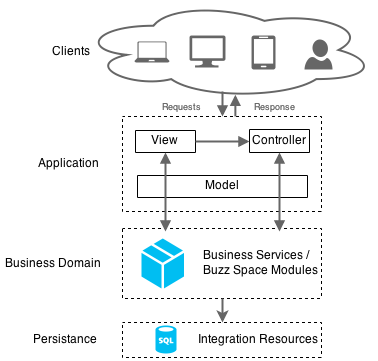
\includegraphics[width=0.85\textwidth]{ReferenceArchitecture}}
	\caption{A basic overview of the buzz space tiered/layered application.}
	\label{fig:refarchandmvc}
\end{figure}
\newpage
\section{Access and Integration Channels}
\subsection{Access Channels}
\subsubsection{Human Access Channels}%Maria
Human Access Channels are all the differnt ways a Human being may interact with and access the Buzz Space.

\begin{enumerate}
	\item The Desktop Computer:
	\begin{itemize}
		\item This will be the most common way for the human (user) to access the Buzz Space on campus. 
		Either at the Information Technoloy labs or the Library.
	\end{itemize}
	\item Laptop:
	\begin{itemize}
		\item A more portable device for the user to access the Buzz Space is with a laptop.
		\item A disadvantage with using ones laptop is that the user will first have to connect to the wifi available to access the Buzz Space.
	\end{itemize}
	\item Mobile Phone:
	\begin{itemize}
		\item Better mobility and portabiliy as the laptop. The user may either connect to the wifi or use his own data to access.
	\end{itemize}
	\item Tablet:
	\begin{itemize}
		\item The last possible human-access-channel is a tablet. It is the same as the mobile phone, the only difference is the screen size of the divice.
	\end{itemize}
\end{enumerate} 
\subsubsection{System Access Channels}%Roger
	System Access Channels is all the external services or applications that have to interact with the Buzz system in some way or another to ensure that all functionality is available to the users. The main systems that will be used in the current project scope are:

\begin{enumerate}
	\item The UP Computer Science Website:
	\begin{itemize}
		\item The Computer Science website must be able to integrate with the system allowing students to access it from module pages providing these users with help and support in their studies.
		\item This system will eventually replace the current outdated CS forum that is being used.
	\end{itemize}
	\item LDAP:
	\begin{itemize}
		\item LDAP is the database used by the University to store and record all of the students information. This database can be modified or expanded to hold user ranks and post information.
		\item This means that access and permissions to the database by the Buzz system need to be provided by the database administrators. 
	\end{itemize}
	\item The Internet:
	\begin{itemize}
		\item Since this system will be integrated with the CS website as mentioned above it will in turn also require access to the Internet allowing students to not only access the system locally but also at home or remotely as mentioned in Human Access Channels.
	\end{itemize}
	\item External Plagiarism Checker:
	\begin{itemize}
		\item Developing a plagiarism checker from scratch is time consuming and also outside the scope of the system so in order to assess the posts for potential copyright infringement access to an external checker will need to be incorporated.
		\item TurnItIn is a company that provides such a service.
	\end{itemize}
\end{enumerate} 
\subsection{Integration Channels}%Sylvester
	\subsubsection*{Channels}
\begin{itemize}
\item The Buzz system will access the CS MySQL database to retrieve information of a particular module/course.
\item The Buzz system will access the CS LDAP server to gain access to and retrieve details of students,  lectures and also a module's enrollment  list.
\end{itemize}

\subsubsection*{Protocols}
The Buzz system will mainly use the HTTPS, LDAP and SMTP protocols.
\begin{itemize}
\item HTTPS: This protocol will be use for security, to ensure that a secure connection is maintained and users information is safe. 
\item LDAP: The protocol that will be used for the integration of the system with the CS LDAP server.
\item SMTP: Notifications for plagiarism or posts not conforming to the netiquette rules will use this protocol for the Buzz email system to enable the communication between the administrator (lecture) and students.  
\end{itemize}
\newpage
\section{Technologies}%Lindelo and Ruth
\subsection{Platform}
\begin{itemize}
		\item Java EE
\end{itemize}


\subsection{Frameworks}
\begin{itemize}
		\item Java Server Faces
\end{itemize}

\subsection{Operating System}
\begin{itemize}
		\item Linux
\end{itemize}
	
	
\subsection{Databases}
\subsubsection{Relational Databases}
\begin{itemize}
	\item MySQL Database
\end{itemize}
	

\subsection{Object Relational Mappers}
\begin{itemize}
	\item JPQL
\end{itemize}

\subsection{Languages}
\subsubsection{Programming Languages}
\begin{itemize}
	\item JavaScript	
	\item Java
\end{itemize}

\subsubsection{Mark-up Languages}
\begin{itemize}
	\item HTML
\end{itemize}


\subsection{Application Servers}
\begin{itemize}
	\item GlassFish Server
	\item Tomcat
\end{itemize}

\subsection{Dependency Management}
\begin{itemize}
	\item Apache Maven
\end{itemize}

\subsection{Web Services}
\begin{itemize}
	\item SOAP-based
\end{itemize} 


\subsection{APIs}
\begin{itemize}
	\item Java Persistence API
\end{itemize}

\begin{itemize}
	\item JAX-RS RESTful web services
\end{itemize}

\begin{itemize}
	\item JAX-WS web service endpoints
\end{itemize}

\begin{itemize}
	\item Java Persistence API entities
\end{itemize}

\begin{itemize}
	\item The Java Database Connectivity API (JDBC)
\end{itemize}

\begin{itemize}
	\item The Java Persistence API
\end{itemize}

\begin{itemize}
	\item The Java EE Connector Architecture
\end{itemize}

\begin{itemize}
	\item The Java Transaction API (JTA)
\end{itemize}


\subsection{Others}
\begin{itemize}
	\item AJAX
\end{itemize}

\begin{itemize}
	\item Servlets
\end{itemize}

\begin{itemize}
	\item Java Server Pages
\end{itemize}


\begin{itemize}
	\item JavaServer Faces
\end{itemize}

\begin{itemize}
	\item JavaServer Faces Facelets
\end{itemize}

\begin{itemize}
	\item Enterprise JavaBeans (enterprise bean) components
\end{itemize}

\begin{itemize}
	\item Java EE managed beans
\end{itemize}


\section{Recommended Technologies}
\subsection{Databases}
\subsubsection{Object Relational Databases}
\begin{itemize}
	\item Postgresql
\end{itemize}

\subsubsection{NoSQL Databases}
\begin{itemize}
	\item Neo4j
	\item MongoDB
\end{itemize}

\subsection{Object Data Mappers}
To cater for the use of NoSQL Databases
\begin{itemize}
	\item Hibernate OGM
\end{itemize}


\end{document}
